% !TeX program = xelatex

\documentclass[landscape,twocolumn,a5paper]{manual}
\usepackage[margin=0.33in,bottom=0.5in,footskip=0.25in]{geometry}

\definecolor{themered}{HTML}{8B3232}
\colorlet{theme}{themered}

\pluginname{ChowTape}

\def\pluginfolder{\href{https://help.uaudio.com/hc/en-us/articles/210216306-Default-Install-Locations-for-UAD-Plug-Ins}{plugin folder}}
\def\dllink#1{\href{https://github.com/jatinchowdhury18/AnalogTapeModel/releases}{#1}}

\begin{document}

\section{ChowTape User Manual}

\noindent
\boldtheme{ChowTape} is an analog tape machine physical model,
originally based on the Sony TC-260. The current version
can be used to emulate a wide variety of reel-to-reel tape
machines. As well as a tool for mixing engineers and producers,
ChowTape is a research project on developing physics-based
models of analog tape emulation\footnote{The plugin is based off a 2019 DAFx paper
\href{http://dafx2019.bcu.ac.uk/papers/DAFx2019_paper_3.pdf}{``Real-time Physical Modelling for Analog Tape Machines''}.}.
The plugin is currently available as VST/VST3/AU/LV2/AUv3 for
Windows, Linux, Mac, and iOS.

\subsection{Installation}
To install ChowTape for desktop, download the plugin installer
from the \href{https://chowdsp.com/products.html#tape}{ChowDSP website}.
If you would like to try the latest changes (unstable), you can
download the latest \href{https://chowdsp.com/nightly.html}{Nightly build}.
It is also possible to compile the plugin
\href{https://github.com/jatinchowdhury18/AnalogTapeModel/blob/master/BUILDING.md}{from the source code}.
ChowTape for iOS can be downloaded from the \href{@TODO}{App Store}.

\begin{figure}[ht]
    \center
    \includegraphics[width=0.45\columnwidth]{../Refs/Pictures/sony_tc-260.jpg}
    \caption{\label{TapeMachine}{\it A Sony TC 260 reel-to-reel tape machine}}
\end{figure}

\begin{figure}[ht]
    \center
    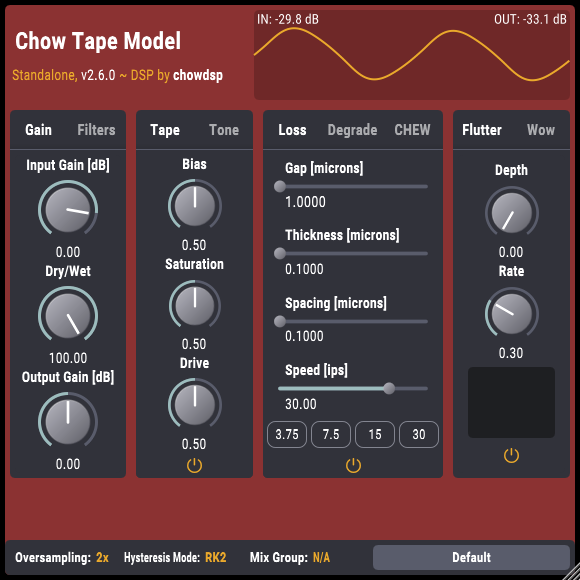
\includegraphics[width=0.55\columnwidth]{../Plugin/Screenshots/full_gui.png}
    \caption{\label{full_gui}{\it ChowTape User Interface}}
\end{figure}

\subsection{Controls}
ChowTape contains a wide range of controls allowing the
user to design the the physical characteristics of the tape
machine and magnetic tape being emulated. Several of the
controls even allow the user to achieve more ``extreme''
results than would be possible with a physical tape machine.

\subsubsection{Main Controls}
\boldtheme{Input Gain} controls the gain level going into the
rest of the plugin. Note that abnormally large levels can
cause the plugin to become unstable, so it is recommended
that sound levels are below unity gain going into the plugin,
and any extra gain should come from the input gain control. %@TODO: more notes on stability
\newpar
\boldtheme{Dry/Wet} allows the user to choose how much of the
signal they want to the plugin's processing to affect.
\newpar
\boldtheme{Output Gain} controls the level coming out of the plugin.
\newpar
\boldtheme{Oversampling} controls the amount of oversampling
being done internally within the plugin. More oversampling
will result in a higher quality sound with fewer aliasing
artifacts and better noise characteristics, but will also
use more CPU. It is recommended to use as much oversampling
as your CPU will allow.
\newpar
\boldtheme{Mix Group}: When using ChowTape on multiple channels
in a mix, you can synchronize parameters between plugin
instances belonging to the same mix group. Essentially, all
the plugin instances in the same mix group will share the same
parameters.

\begin{figure}[ht]
    \center
    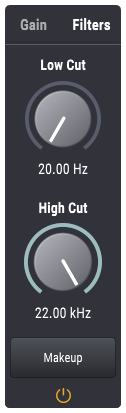
\includegraphics[height=0.32\paperheight]{../Plugin/Screenshots/Filters.png}
    \caption{\label{h_bias}{\it Input filter controls}}
\end{figure}

\subsubsection{Input Filter Controls}
The ChowTape input filters apply a low-cut and high-cut filter
to the input signal before it is passed on to the rest of the
plugin. The \boldtheme{Low Cut} and \boldtheme{High Cut} knobs
control the cutoff frequencies of the two filters. The
\boldtheme{Makeup} control allows the signal cut out by the
input filters to be added back to the output of the plugin.
This can be useful for allowing sub-bass frequencies to pass
through the plugin unaffected.

\begin{figure}[ht]
    \center
    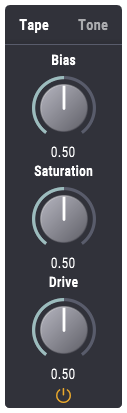
\includegraphics[height=0.35\paperheight]{../Plugin/Screenshots/Tape.png}
    \caption{\label{h_bias}{\it Tape hysteresis controls}}
\end{figure}
%
% \begin{figure}[ht]
%     \center
%     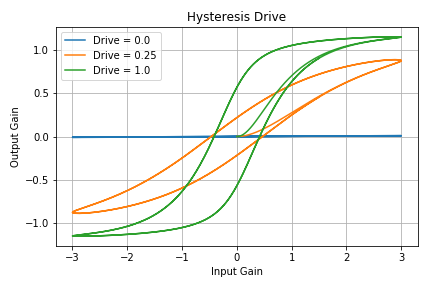
\includegraphics[width=0.9\columnwidth]{../Simulations/Hysteresis/drive.png}
%     \caption{\label{h_drive}{\it Hysteresis curves with varying drive}}
% \end{figure}
%
\begin{figure}[ht]
    \center
    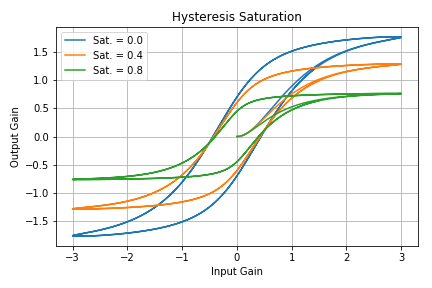
\includegraphics[width=0.85\columnwidth]{../Simulations/Hysteresis/sat.png}
    \caption{\label{h_sat}{\it Hysteresis curves with varying saturation}}
\end{figure}
%
\begin{figure}[]
    \center
    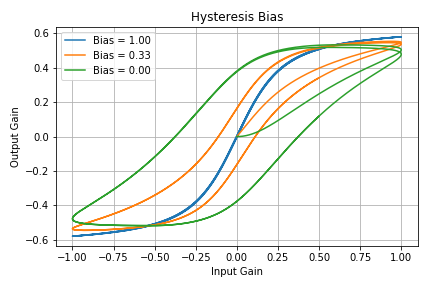
\includegraphics[width=0.85\columnwidth]{../Simulations/Hysteresis/bias.png}
    \caption{\label{h_bias}{\it Hysteresis curves with varying bias}}
\end{figure}

\subsubsection{Hysteresis Controls}
The hysteresis processing is the most important section of the
plugin. \href{https://en.wikipedia.org/wiki/Hysteresis}{Hysteresis}
is a complex nonlinear phenomenon that describes many
natural processes in physics, biology, economics, and more.
In particular, magnetic hysteresis describes the process by
which tape becomes magnetised when subjected to a strong magnetic
field. ChowTape emulates magnetic hysteresis, using the
Jiles-Atherton\footnote{Jiles, D.C.; Atherton, D.L. (1984) ``Theory of ferromagnetic hysteresis'' \textit{Journal of Applied Physics}.}
model of magnetic hysteresis. Magnetic hysteresis is largely
responsible for the ``warm'' sound often associated with
analog tape distortion.
\newpar
\boldtheme{Drive} controls the level of amplification done by
the hysteresis process. This differs from the input gain in that
it affects the nonlinear characteristic of the hysteresis process.
\newpar
\boldtheme{Saturation} controls the level at which the hysteresis
function saturates. Higher values correspond to a lower Saturation
point, resulting in a more distorted sound.
\newpar
\boldtheme{Bias} controls the amount of bias used by the tape
recorder. Tape bias is the addition of an inaudible high-frequency
signal to the audio signal\footnote{\href{https://hccc.org.uk/acbias.html}{More information on tape biasing}}.
At lower bias levels, the hysteresis curve becomes ``wider'',
thus creating the ``deadzone'' effect often associated with
underbiased tape.
\newpar
\boldtheme{Hysteresis Mode} selects the equation solver used
to solve the Jiles-Atherton equation in real time. ChowTape
currently supports the following hysteresis modes:
\renewcommand{\labelitemi}{\textendash}
\begin{itemize}
    \itemsep-1mm
    \item 2nd-order Runge Kutta (RK2)
    \item 4th-order Runge Kutta (RK4)
    \item 4-iteration Newton Raphson (NR4)
    \item 8-iteration Newton Raphson (NR8)
    \item State Transition Network\footnote{Parker, J.D. et. al. (2019) ``Modelling of Nonlinear State-Space Systems using a Deep Neural Network'' \textit{Proc. 22\textsuperscript{nd} Int. Conference on Digital Audio Effects}.} (STN)
    \item Version 1.0 processing (V1)
\end{itemize}
%
The Runge-Kutta solvers are computationally cheaper, but
somewhat less accurate than the Newton-Raphson solvers.
Similarly, the higher-order solvers will be more accurate,
but will also consume more compute resources. The State
Transition Network is designed to be a computationally
cheaper approximation of the NR8 solver; although it
distorts more harshly at extreme settings. The V1 mode
reverts to a different parameterization of the hysteresis
equation that was used in earlier versions of the plugin. It
is recommended to use higher-order solvers for mix busses
and key tracks in a mix, while using lower-order solvers for
less important tracks.

\subsubsection{Tone Controls}
The tone section applies a set of pre-/post-emphasis filters
to the signal before and after the hysteresis processing
is applied. The filters work similar to
\href{https://en.wikipedia.org/wiki/RIAA_equalization}{RIAA filters},
in that the pre- and post- filters have exact opposite frequency
responses.
\newpar
The \boldtheme{Bass} and \boldtheme{Treble} knobs control
the frequency response of the pre-emphasis filter, and the
post-emphasis filter will automatically adjust. The
\boldtheme{Frequency} knob controls the transition frequency
between the bass and treble sections of the filter.

\begin{figure}[ht]
    \center
    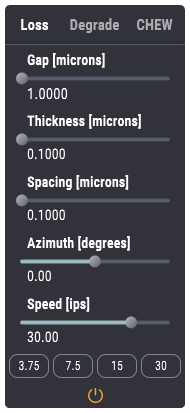
\includegraphics[height=0.32\paperheight]{../Plugin/Screenshots/Loss.png}
    \caption{\label{h_bias}{\it Loss filter controls}}
\end{figure}
%
\begin{figure}[ht]
    \center
    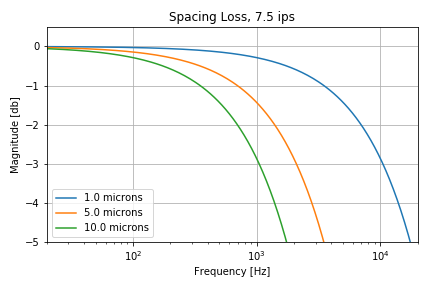
\includegraphics[width=0.85\columnwidth]{../Simulations/LossEffects/space_loss.png}
    \caption{\label{spacing_loss}{\it Spacing loss at 7.5 ips}}
\end{figure}
%
\begin{figure}[ht]
    \center
    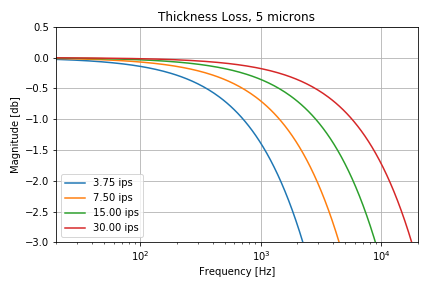
\includegraphics[width=0.85\columnwidth]{../Simulations/LossEffects/speed_thickness.png}
    \caption{\label{thick_loss}{\it Thickness loss for 5 micron tape}}
\end{figure}

\subsubsection{Playhead Controls}
Physical tape machines also have a frequency response that
is affected by the amount of space between the playhead and
the tape, the width of the playhead gap, and the thickness
of tape used. The frequency responses of each of these ``loss
effects'' is also dependent on the tape speed.
\newpar
\boldtheme{Spacing}
controls the amount of space between the playhead and the tape,
measured in centiimeters.
\newpar
\boldtheme{Thickness} controls the thickness
of the tape, measured in centiimeters.
\newpar
\boldtheme{Gap} controls
the width of the playhead gap, measured in millimeters.
\newpar
\boldtheme{Azimuth}
controls the playhead alignment angle\footnote{\href{https://blog.weareavp.com/azimuth-adjustment-for-magnetic-audio-recordings}{More information on playhead azimuth}.}.
A misalignment between the playhead and the tape causes a
corresponding time misalignment between the two stereo tracks
on the tape, resulting in a stereo ``widening'' effect.
\newpar
\boldtheme{Speed}
controls the tape speed as it effects the above loss effects,
measured in inches per second (ips). While this control is
continuous, the parameter can be quantized to the standard speeds
for reel-to-reel tape machines: 3.75, 7.5, 15, and 30 ips.


\subsubsection{Tape Degradation Controls}
The degradatation parameters control a simulation of
old tape that has been used over and over, and has started
to degrade.
\newline
\boldtheme{Depth}
controls the intensity of the wear on the tape. Enable the
\boldtheme{0.1x} option to make this control more subtle.
\newpar
\boldtheme{Amount}
controls the amount of wear, typically corresponding to
the age of the tape.
\newpar
\boldtheme{Variance}
adds a time-varying randomness to the degradatation.
\newpar
\boldtheme{Envelope}
applies an amplitude envelope to the tape noise.

\begin{figure}[ht]
    \center
    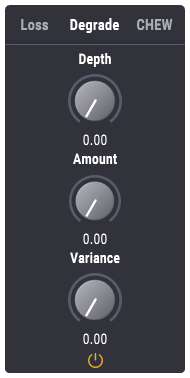
\includegraphics[height=0.32\paperheight]{../Plugin/Screenshots/Degrade.png}
    \caption{\label{h_bias}{\it Degradation controls.}}
\end{figure}

\subsubsection{Chew Controls}
The chew parameters simulate tape that has been chewed up by
a broken tape machine. \boldtheme{Depth} controls how deep the
tape is chewed, \boldtheme{Frequency} controls how much space
there is between bits of tape that have been chewed up, and
\boldtheme{Variance} determines how much randomness there is
in determining the amount of space between chewed up sections.

\subsubsection{Wow and Flutter Controls}
Tape machines also exhibit timing irregularities, often due
to small imperfections in the mechanics of the machine causing
the tape to subtly speed up and slow down while being
played back. The flutter characteristic in this plugin was
captured from an original Sony TC-260 tape machine.
\newpar
%
\begin{figure}[ht]
    \center
    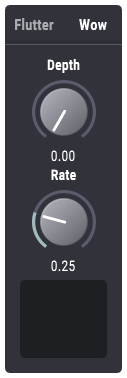
\includegraphics[height=0.32\paperheight]{../Plugin/Screenshots/Wow.png}
    \caption{\label{h_bias}{\it Wow controls.}}
\end{figure}
%
\boldtheme{Depth} controls the depth of the flutter and
\boldtheme{Rate} controls the rate of flutter, with higher values
causing the flutter to occur faster. Note that the
flutter rate can be synchronized to the tape speed, or to the
tempo of the song.
\newpar
"\boldtheme{Wow}" is similar to flutter but on a much longer time scale,
and contains similar controls, as well as \boldtheme{Variance} and
\boldtheme{Drift} which control the random irregularities that
cause the wow characteristic.

\subsection{Presets}
Presets provide a quick way to achieve a specific sound
with the plugin. ChowTape comes with a set of built-in
factory presets. To contribute your presets to be added
to the factory presets list for future releases, see the
\href{https://github.com/jatinchowdhury18/AnalogTapeModel/issues/30}{Presets GitHub issue}.

\subsubsection{User Presets}
To save the current plugin state as a user preset, open
the presets menu, and select ``Save''. The first time a
preset is saved, you will be asked to choose a preset
folder. All future presets will be saved to this folder,
and when the plugin opens, it will search this folder, as
well as any subfolders, to load new user presets.
Presets located in subfolders will be placed in their
own groups in the preset menu.

\subsection{Open Source}
ChowTape is open-source software that is free (as in ``free
beer''), and free (as in ``free speech''), under the
\href{https://www.gnu.org/licenses/gpl-3.0}{General Public License}.
As a research project, the goal of developing this plugin is
to help advance the body of knowledge of real-time audio
signal processing. Therefore, keeping any part of this project
behind a paywall, or licensing this software under a proprietary
license would be antithetical to that goal. As an open-source
project, ChowTape is open to outside contributors. For more
information, see our
\href{https://github.com/jatinchowdhury18/AnalogTapeModel/blob/master/CONTRIBUTING.md}{Contributing}
page.

\subsection{Feedback}
If you notice any bugs, or have any questions, feel free
to \href{mailto:chowdsp@gmail.com}{email me directly},
or \href{https://github.com/jatinchowdhury18/AnalogTapeModel/issues}{create an issue ticket}
on GitHub. GitHub issues are preferred, since they are publicly
visible.

\vspace{8em}

\subsection{Acknowledgements}
Thanks to Yann from SINK Music for helping to create this
user manual, as well as all the users of ChowTape who have
made efforts to help improve the plugin.
\newpar
Enjoy!
\newpar
Jatin Chowdhury
\newpar
\href{https://github.com/jatinchowdhury18/AnalogTapeModel}{https://github.com/jatinchowdhury18/AnalogTapeModel}

\end{document}
